\subsection{Relays and Transistors} 

Answers to M\Alph{subsection} problems are on page \pageref{relays_transistors_prob_answers}.  \textbf{\textcolor{red}{Updated \DTMnow.}}

%--------------------------------------------------------------------------------------------------------------
\begin{Exercise}
Look at the Wikipedia entry for ``switch''.  

\figuretoright{0.23}{M_problems/relays_transistors/MBB_SP4T.pdf}{
\begin{enumerate}[nosep, label=(\alph*),nosep]
\item What is meant by \textit{shorting} switches and \textit{non-shorting} switches? 
\item What is the meaning of the abbreviations BBM and MBB? 
\item The picture to the right is a symbol a four-position (SP4T) MBB rotary switch.  Draw a similar symbols for an MBB SPDT switch and an MBB DPDT switch.
\item Based on the graphs you drew in 
Lab~\ref{lab_relays}, parts~\ref{part_connecting_relay_coil} and~\ref{part_disconnecting_relay_coil},
 is your DPDT relay an MBB or BBM switch?
\end{enumerate}
}
\begin{enumerate}[resume,label=(\alph*),nosep,start=5]
\item Redraw what your graphs from  
Lab~\ref{lab_relays}, parts~\ref{part_connecting_relay_coil} and~\ref{part_disconnecting_relay_coil}
would look like if your DPDT relay were the \textit{other} type of switch (that is, BBM instead of MBB, or MBB instead of BBM).
\end{enumerate}
\end{Exercise}


%--------------------------------------------------------------------------------------------------------------
\begin{Exercise}
\label{prob_superposition_diode}
In the circuit below, the Zener diode has $V_F=0.7$~V and $V_R=3.2$~V. (a)~Find the instantaneous current through resistor $R_1$ at the time of (a)~the peak positive source voltage of $+5$ volts, and (b)~the peak negative source voltage of $-5$~volts.  Hint: To analyze the circuit in the case that you assume $I_\text{diode} \neq 0$, treat the diode as a second voltage source, oriented against the direction of current flow.  Then analyze the circuit using the principle of superposition as you did in problem~\ref{prob_superposition}.
\begin{center}
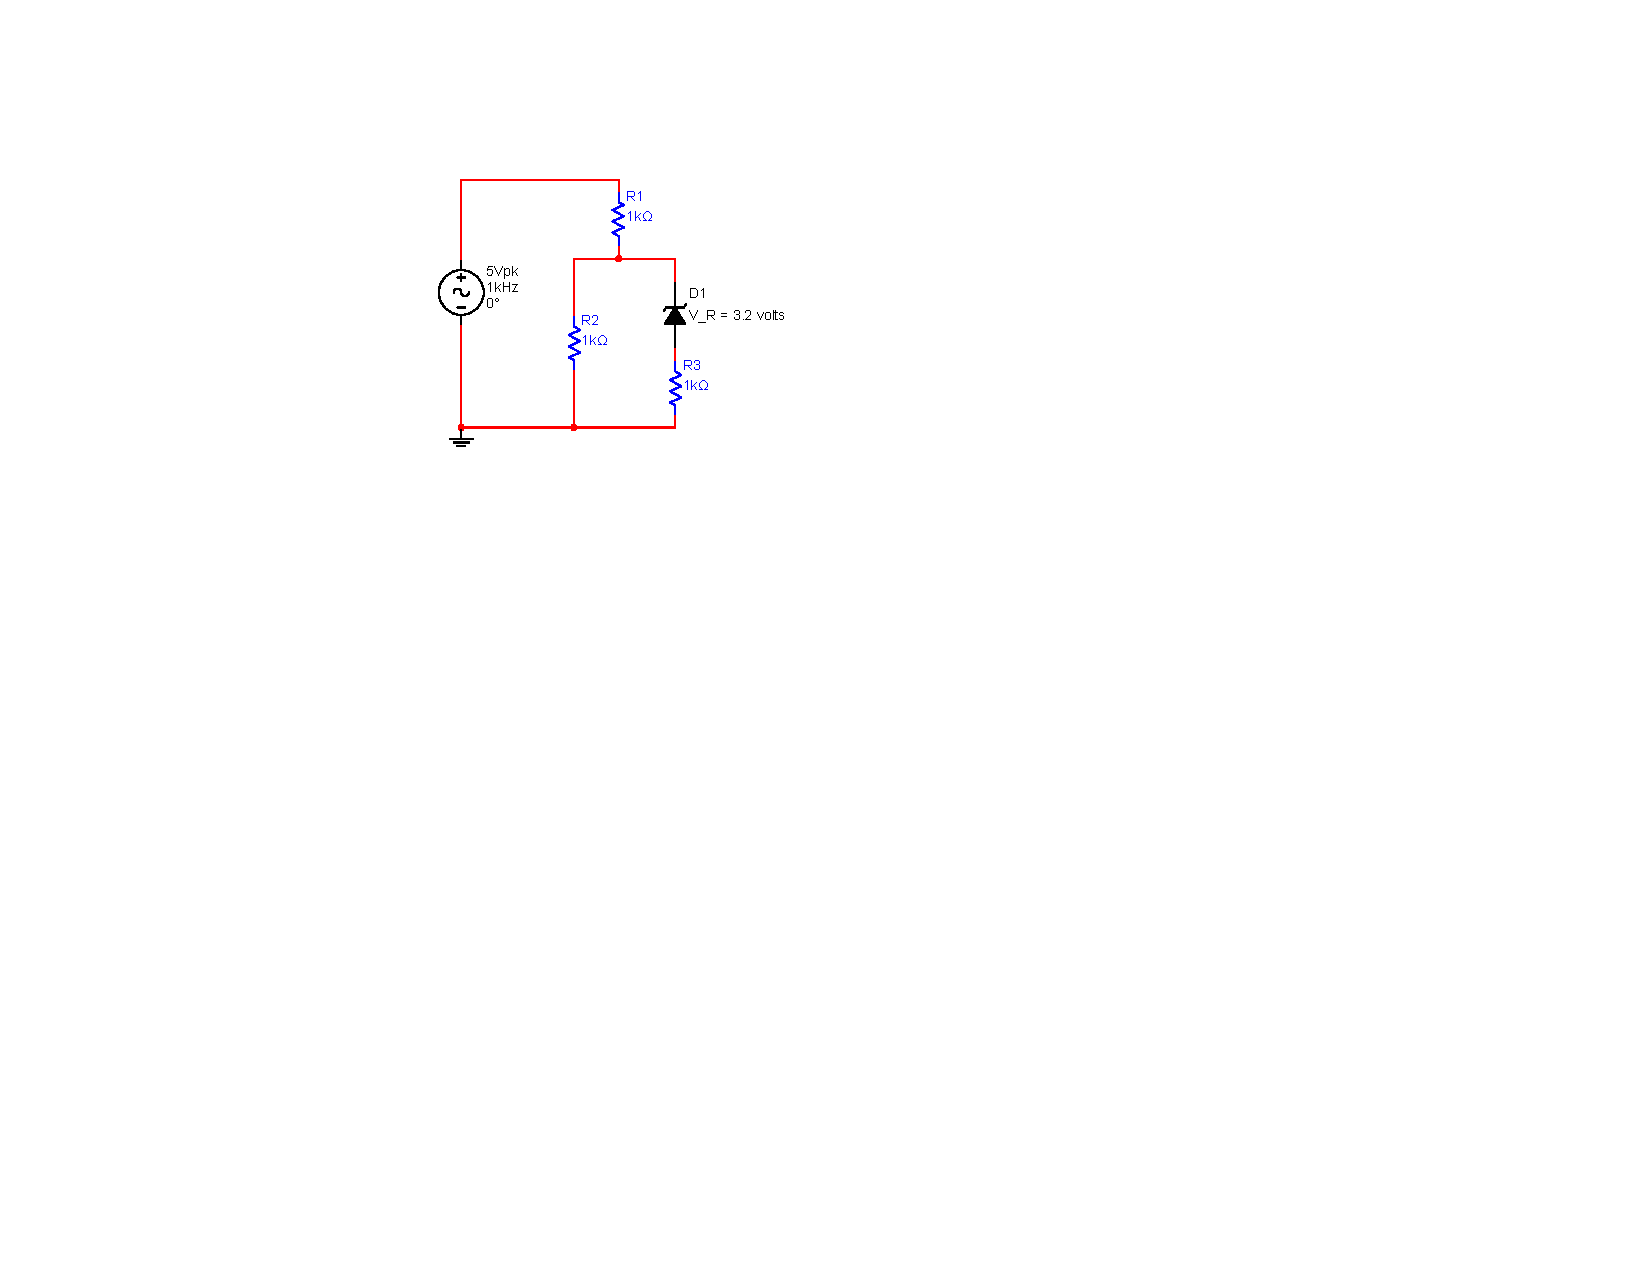
\includegraphics{M_problems/relays_transistors/diode_circuit_with_superposition.pdf}
\end{center}
\end{Exercise}
\begin{Answer}
(a) 2.5 mA (b) $-3.1$~mA.  Hint: if you got 2.27~mA for part (a), you probably assumed that there is current through the diode, so that the voltage across it is 3.2~V.  But as you learned in problem~\ref{prob_first_diode_resistor_with_steps}, it's also possible that there is no current through the diode.  One of these scenarios leads to a physically plausible solution, and the other does not; you'll need to try both to see which one is correct.
\end{Answer}


%--------------------------------------------------------------------------------------------------------------
\begin{Exercise}
In this problem, we'll use a series of successive approximations to find the DC level of $V_B$ (also sometimes called the \textit{quiescent} value of $V_B$) for the circuit below on the left.  (a)~Find $V_B$ making the approximation $I_B=0$.  (b)~Find $V_B$ acknowledging that $I_B>0$, but assuming $\Delta V_\text{BE} \approx 0$ and  treating $R_E$ as an equivalent resistance $R_\text{eq}$ in parallel with $R_2$, where $R_\text{eq} = h_\text{FE} R_E$.  (c)~Find $V_B$ using the equivalent circuit below on the right, where $R_\text{eq} = h_\text{FE} R_E$ and we use diode D1 to model $\Delta V_\text{BE}$.  (To find $V_B$ for this equivalent circuit assume D1 has $V_\text{F}=0.7$~V, and use the method of superposition as you did in problems \ref{prob_superposition} and \ref{prob_superposition_diode}.) 

\hspace{\fill}
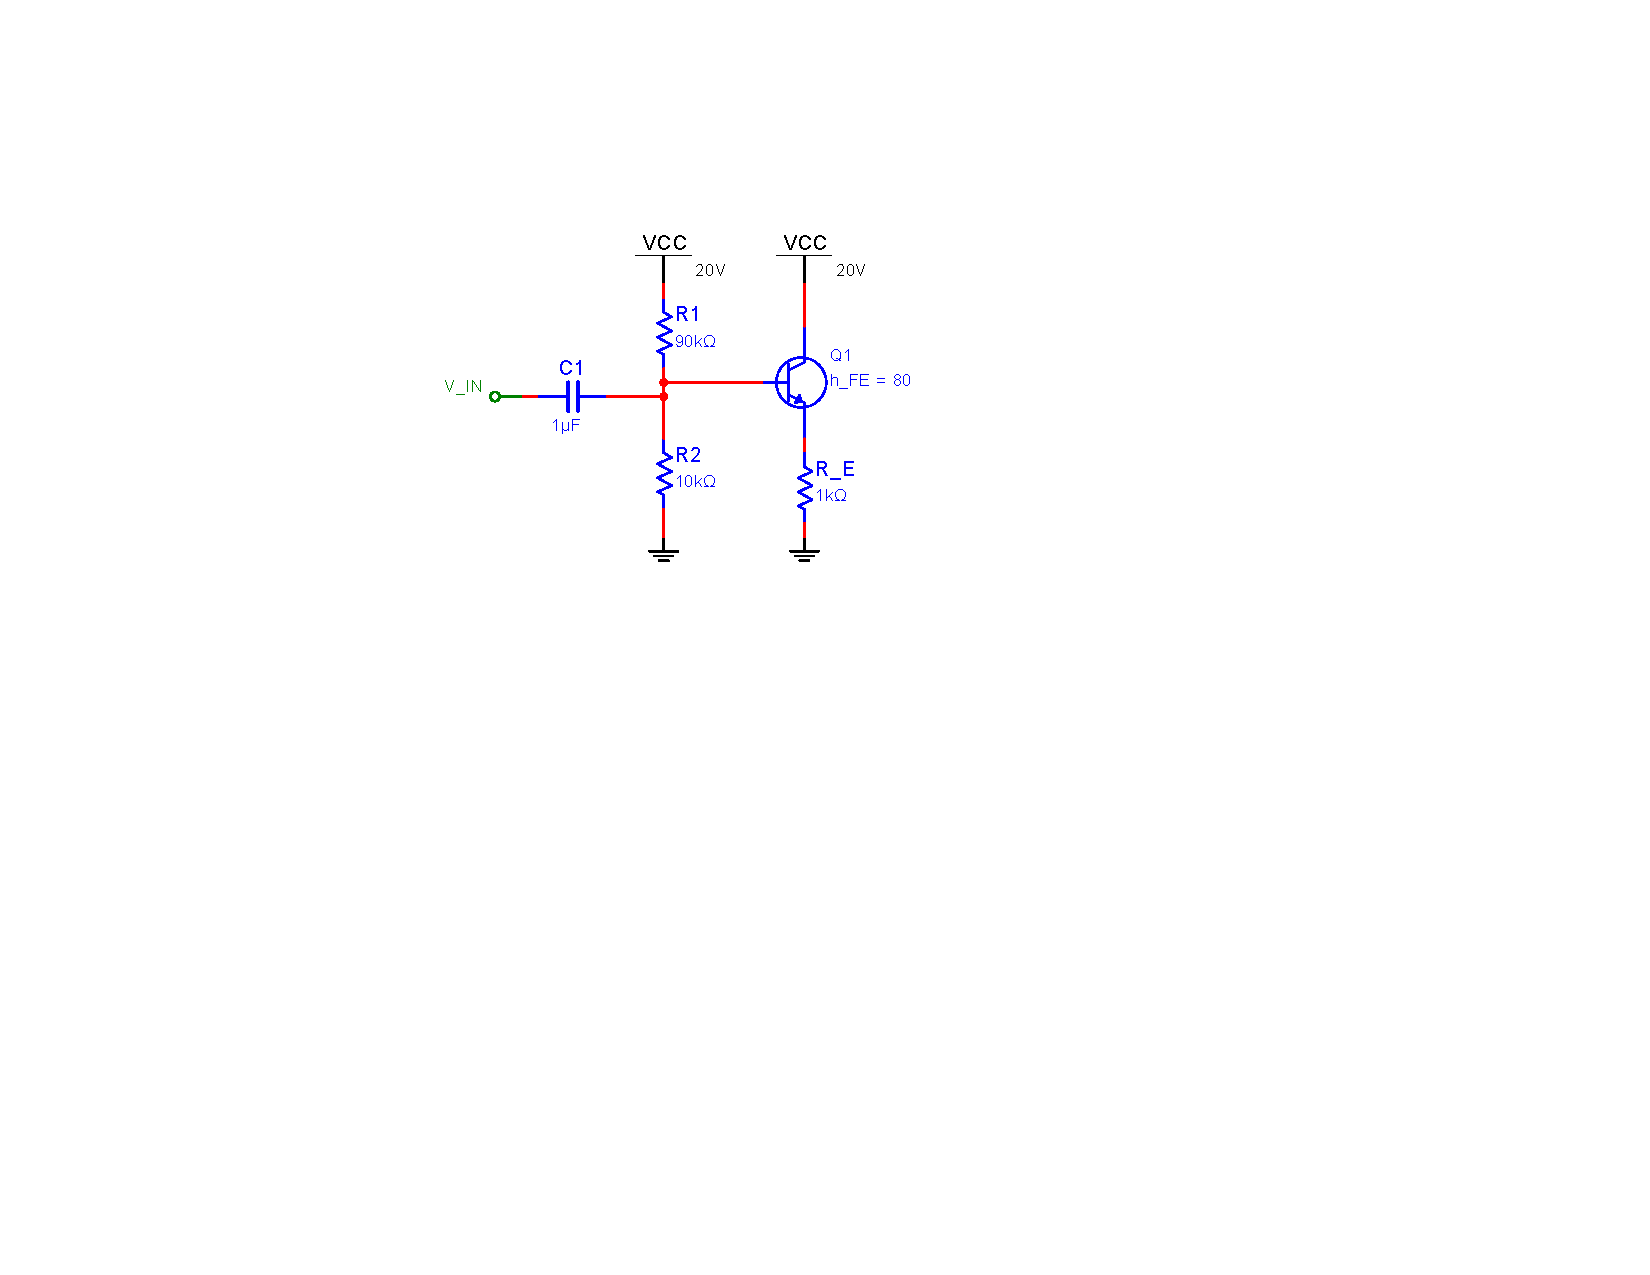
\includegraphics[scale=0.8]{M_problems/relays_transistors/R_E_models_part_a.pdf}
\hspace{\fill}
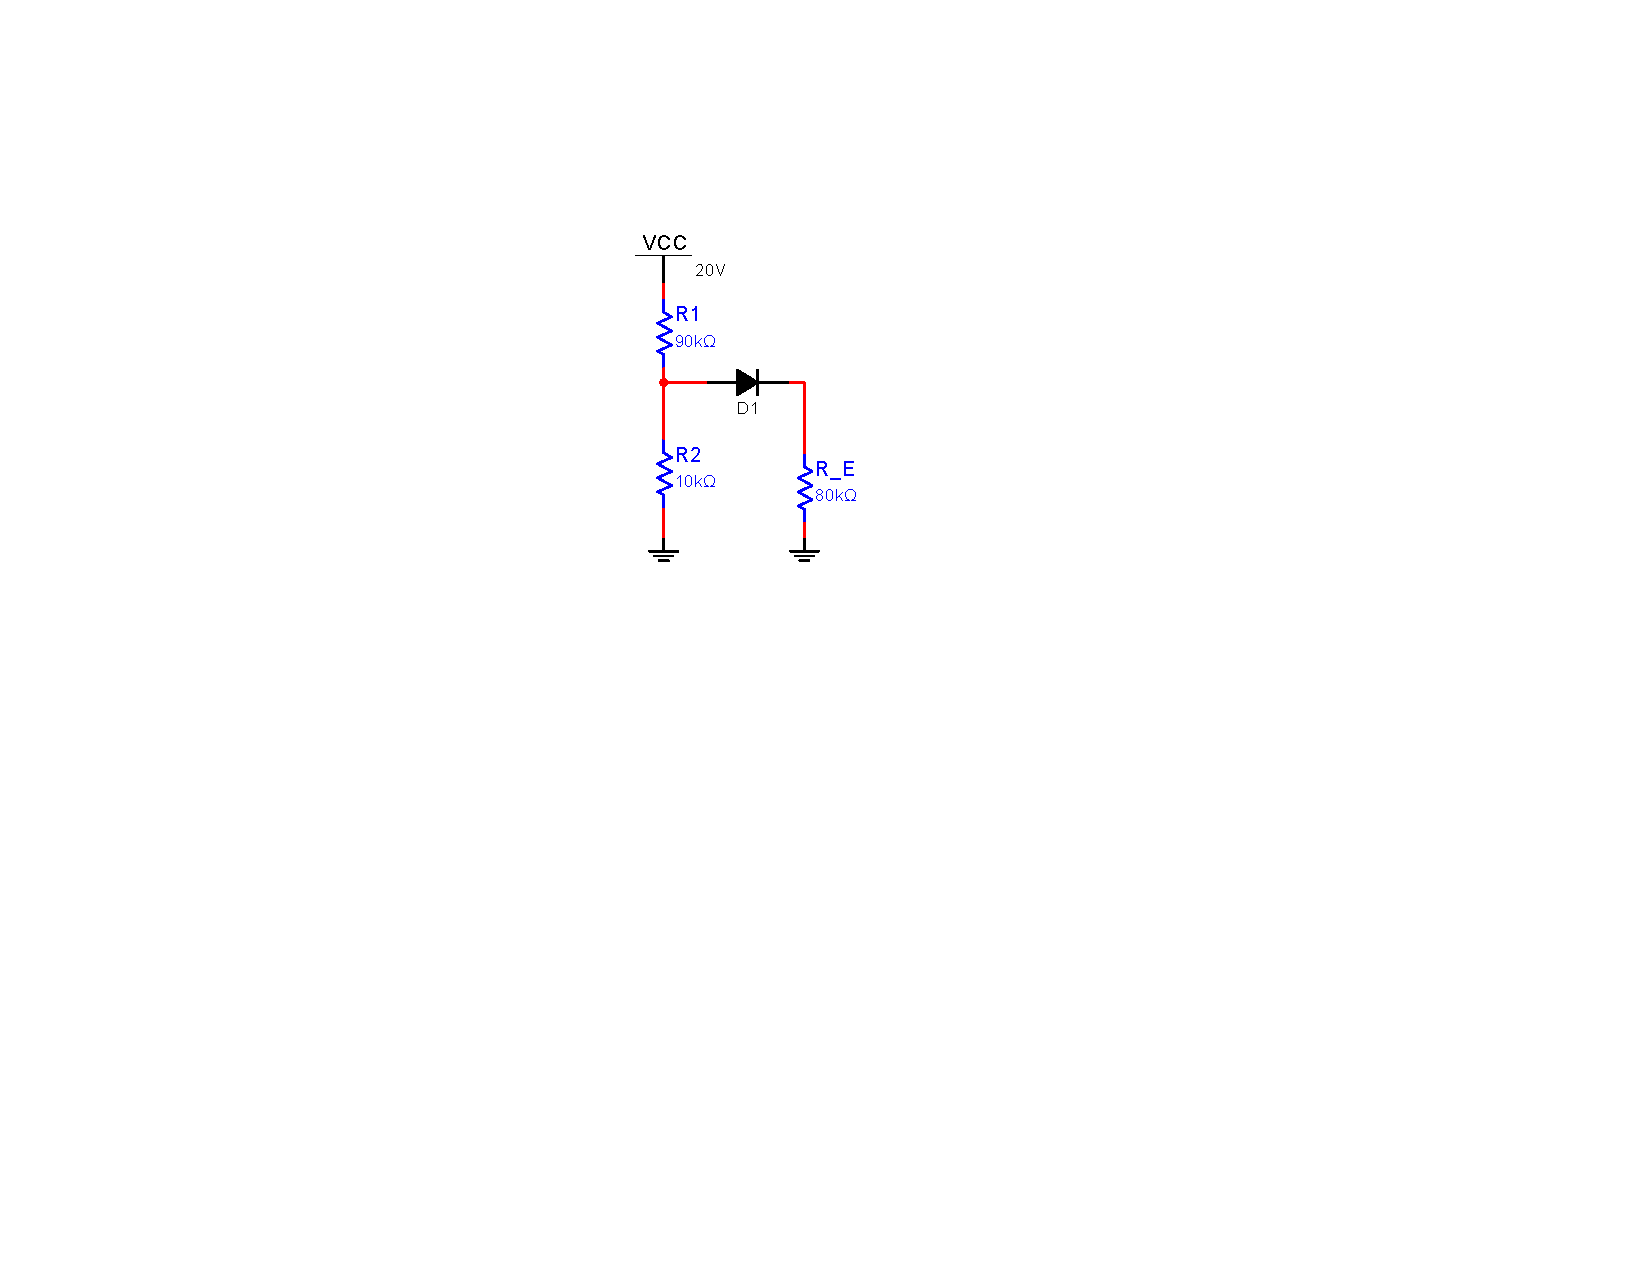
\includegraphics[scale=0.8]{M_problems/relays_transistors/R_E_models_part_c.pdf}
\hspace*{\fill}
\end{Exercise}
\begin{Answer}
(a) 2 V (b) 1.80 V (c) 1.87 V
\end{Answer}


\pagebreak[4]
%--------------------------------------------------------------------------------------------------------------
\begin{Exercise}
\label{prob_Linda_Swintayla}
In the circuit shown, the transistor is used as an emitter follower amplifier to provide current to the load resistor.  
\figuretoright{0.20}[scale=0.8]{M_problems/relays_transistors/bjt_power.pdf}{
\begin{enumerate}[nosep, label=(\alph*)]
\item Calculate both the power $P_R$ dissipated in the load resistor and the power $P_T$ dissipated in the transistor for input voltages of $V_\text{in}= 0$~V, 5.7~V, and 9.7~V.  For which input voltage is $P_T$ greatest?
\end{enumerate}

\medskip
Lin-Manuel Miranda and Taylor Swift have much in common, as both are grammy-award-winning musicians with mutual admiration for each other's work.  In this problem, they are each designing custom power supplies that will convert a high voltage input into a low voltage DC output used to power a computer board.  Lin-Manuel (known as ``Lin'' to family and friends) has designed a circuit that will smoothly adjust the current through a transistor to maintain a constant output voltage at its emitter.  By contrast, Ms. Swift's circuit will cycle the transistor quickly between zero current and maximum current, storing energy during part of the cycle and drawing that stored energy down for the rest of the cycle to supply power to the load.  
}
\begin{enumerate}[nosep, label=(\alph*),nosep,start=2]
\item Based on the numbers you calculated in part (a), is Lin's power supply or Ms. Swift's power supply likely to be more efficient, dissipating less power in the transistor?  
\item Whose power supply is likely to have lower noise (i.e. lower ripple voltage)---Lin's or Ms. Swift's?  
\item Read at least the first few paragraphs of the article entitled ``switched-mode power supply'' on Wikipedia.  Why were Lin and Ms. Swift chosen as the characters in this problem?
\end{enumerate}
\end{Exercise}
\begin{Answer}
(a) Greatest for 
$V_\text{in}=5.7$~V, for which $P_T=2.5$~W 
(b)~Swintayla's is probably more efficient.  
(c)~Linda's is probably smoother.  
(d)~Hint: What types of power supplies did \textbf{\underline{Lin}}-Manuel Miranda and Taylor \underline{\textbf{Swi}}ft each design?
\end{Answer}

%--------------------------------------------------------------------------------------------------------------
\begin{Exercise}
The circuit below is a two-stage amplifier made from three 2N3904 transistors with $h_\text{FE}=160$.  
(a)~What is the cutoff frequency of the filter that uses capacitor $C_1$?  
(b)~Is it a high pass filter or a low pass filter?  
(c)~What are the DC voltages at the base, emitter, and collector of the first transistor, $Q_1$?  (d)~What is the DC current into the base of transistor $Q_1$?  
(e)~What is the AC voltage gain of the first amplifier stage?  
(f)~What is the purpose of the second amplifier stage, made by transistors $Q_2$ and $Q_3$?  
(g)~What is the AC voltage gain of this stage?  
(h)~What is the DC current into the base of transistor $Q_2$? 

\begin{center}
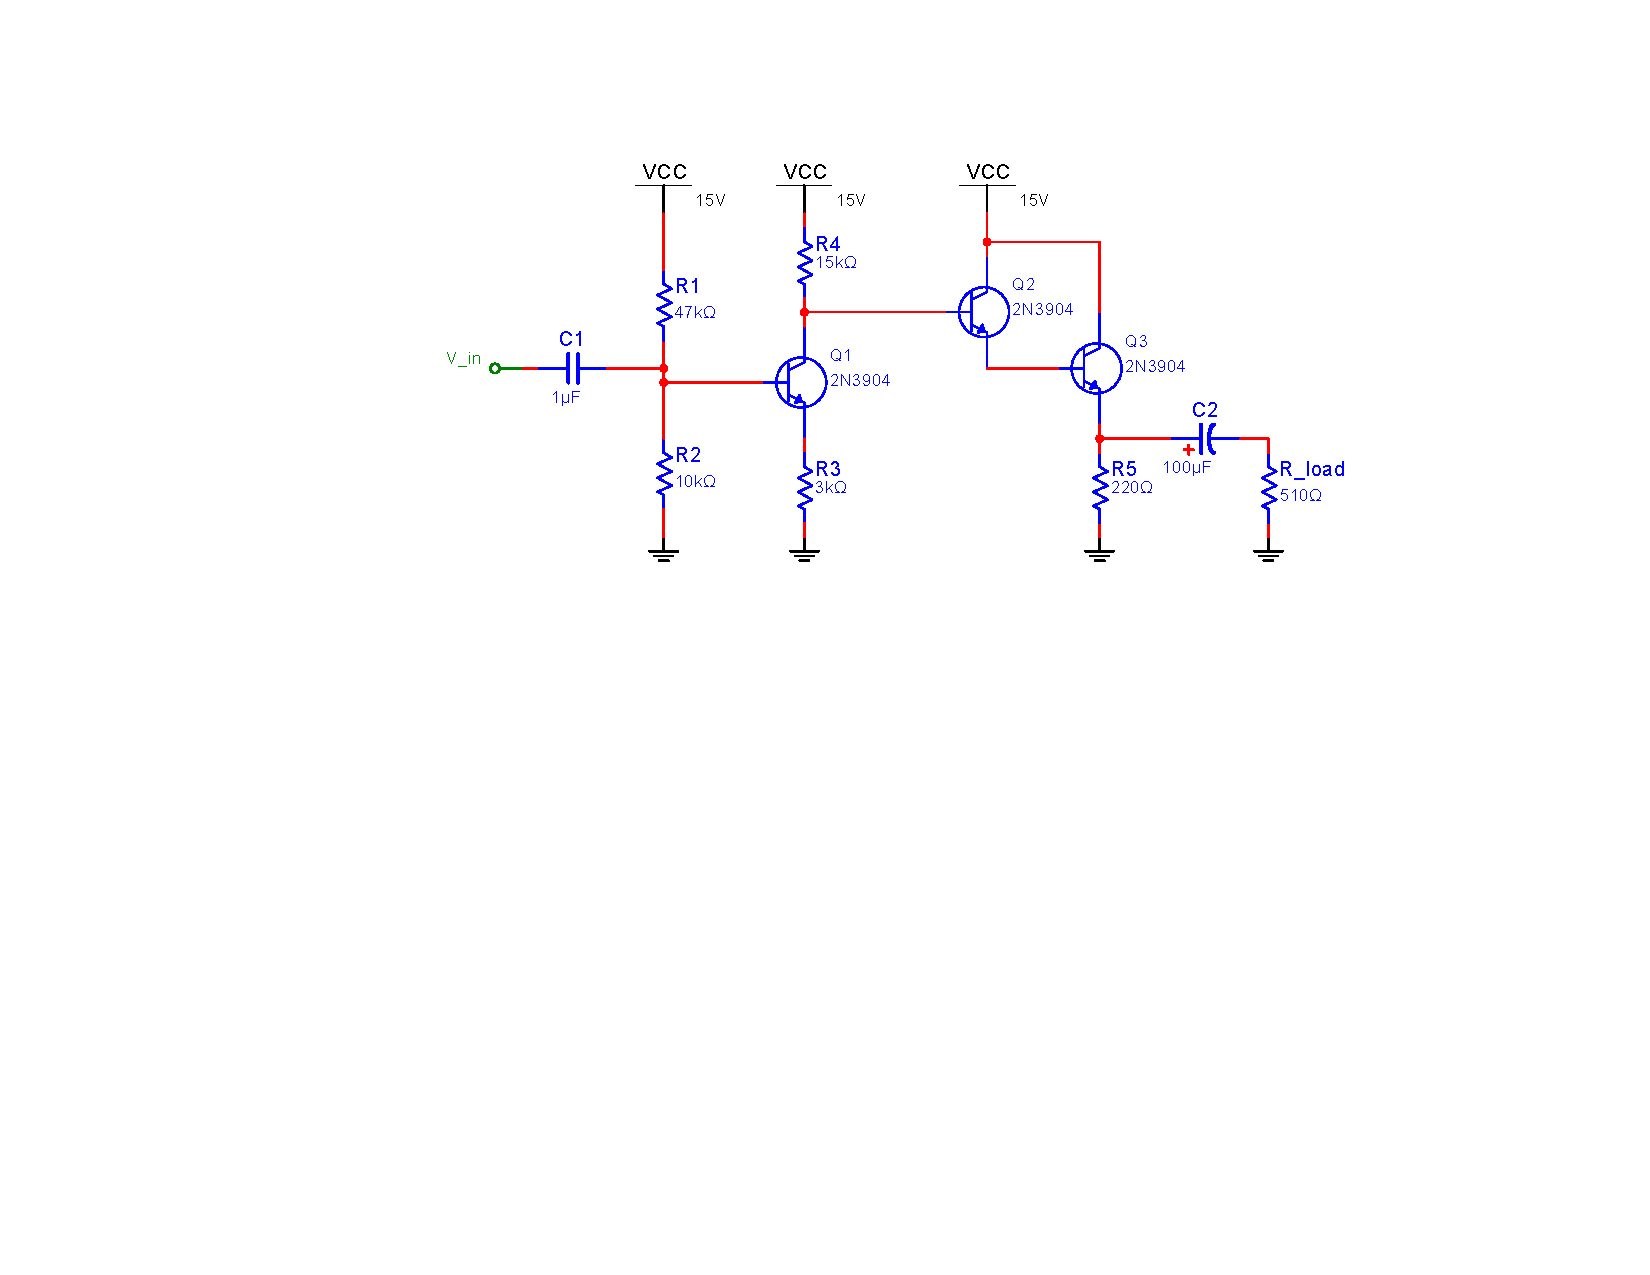
\includegraphics[scale=0.8]{M_problems/relays_transistors/bjt_two_stage_amplifier.pdf}
\end{center}

\end{Exercise}
\begin{Answer}
(a) 19.3 Hz (b) High pass (c) 2.63 V, 1.93 V, 5.35 V (d) 4.0 $\mu$A (e) $-5$ (f) ``Current Gain,'' allowing the amplifier to work with smaller load resistances.  (g)~1 (h)~700~nA
\end{Answer}

%Ideas for additional problems:
%\vfill
%\pagebreak[3]

\vspace{0.7in}

\textbf{Answers to Selected {\thesubsection} Problems:}
\label{relays_transistors_prob_answers}
%\shipoutExercise
\shipoutAnswer

\cleardoublepage
